\documentclass{article}
\usepackage[utf8]{inputenc}
\usepackage[portuguese]{babel}
\usepackage[a4paper, total={7in, 9in}]{geometry}
\usepackage{graphicx}
\usepackage{float}
\usepackage[title]{appendix}
\usepackage[style=numeric]{biblatex}
\usepackage{csquotes}
\usepackage{mathtools}
\usepackage{fancyvrb}
\addbibresource{references.bib}

\begin{document}

{
\center
\textsc{\Large Universidade do Minho} \\ [0.5cm]
\textsc{\Large Mestrado em Engenharia Informática} \\ [0.5cm]
\textsc{\large Paradigmas de Computação Paralela} \\ [0.5cm]

{\LARGE \bfseries Paralelização de um algoritmo de simulação de ondas sonoras através de códigos stencil} \\[0.5cm]

\begin{tabular}{c c}
    José Carlos Lima Martins & Miguel Miranda Quaresma \\
    A78821 & A77049  \\
\end{tabular} \\[0.5cm]

\today \\[1cm]
}

\section{Introdução}
O desenvolvimento de aplicações paralelas permite a obtenção de níveis de \textit{performance} que não seriam possíveis em aplicações em que a complexidade e quantidade de dados são lineares (ou mesmo superlineares) face ao tamanho do \textit{input}, sendo este o caso de muitas aplicações de cariz científico. Como tal torna-se indispensável o recurso a paradigmas que permitam efetuar estas implementações de maneira sistematizada de modo a desenvolver aplicações com tempos de execução aceitáveis mesmo para tamanhos de \textit{input} consideráveis. O presente trabalho apresenta uma implementação realizada segundo um paradigma de memória partilhada para um código \textit{stencil} de simulação da propagação de ondas sonoras, recorrendo para isso à API 
OpenMP. Inicialmente será apresentada uma breve descrição do problema a resolver, simulação de ondas sonoras através de códigos \textit{stencil}, procedida de uma descrição do contexto de experimentação \textbf{i.e.} hardware e métodos estatísticos 
utilizados sendo ainda referidos os parâmetros usados nos diferentes testes realizados. Por fim serão apresentadas três versões para a implementação, a primeira que serviu de base para as outras duas e que corresponde a uma versão sequencial, uma segunda implementação que recorre a um conjunto de otimizações para extrair o máximo de \textit{performance} da versão sequencial e a terceira versão, o foco deste trabalho, que corresponde à paralelização da versão otimizada com recurso ao OpenMP. Após 
esta descrição é realizada uma análise crítica dos resultados das medições efetuadas para cada uma destas versões. Por fim, na secção \ref{concl}, são apresentadas as conclusões relativamente ao comportamento deste tipo de algoritmos (\textit{stencil}) 
num paradigma de memória partilhada.

\section{Descrição do problema}\label{algorithm}
Os padrões \textit{stencil} são uma classe de algoritmos que possuem um conjunto de aplicações que variam desde a realização de simulações em computador à resolução de sistemas de equações por métodos iterativos ou de autómatos celulares.
Estes padrões funcionam iterativamente atualizando cada valor segundo um padrão fixo de posições na sua vizinhança aplicando, por vezes, uma máscara aos valores destas posições antes de os combinar. Dado serem de complexidade linear face ao tamanho 
do \textit{input} utilizado é de extrema importância paralelizar este tipo de algoritmos por forma a tornar possível a realização de simulações de tamanho considerável. Adicionalmente, dado serem algoritmos que possuem uma elevada utilização da memória,
é necessário gerir esta utilização de forma eficiente por forma a reduzir o impacto da mesma no desempenho da implementação.
O padrão de \textit{stencil} estudado neste trabalho corresponde à simulação da propagação de ondas sonoras usando, para isso, uma vizinhança de 4 pontos em cada direção:
\begin{figure}[H]
    \centering
    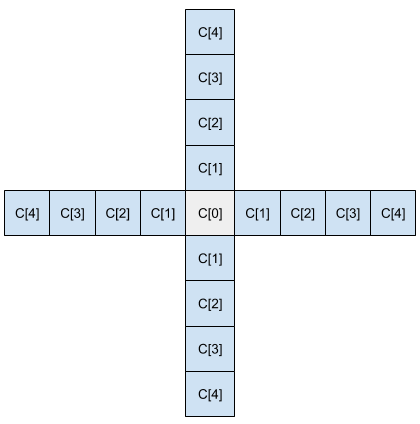
\includegraphics[width=4cm]{Pictures/stencil_abstract_imp.png}
\end{figure}

Em cada instante, o valor central $M_{i,j}$ é atualizado recorrendo à seguinte fórmula, que aplica uma máscara $C$ aos valores dos pontos na sua vizinhança em função da distância dos mesmos ao ponto central:

$$M_{i,j} = \sum_{k=1}^{4} (M_{i,j+k}+M_{i,j-k}+M_{i+k,j}+M_{i-k,j})*C_k + M_{i,j}*C_0$$

Dado o tamanho da vizinhança ser de 4 pontos, a presente implementação assume uma margem de 4 pontos no início e fim de cada coluna/linha que se mantém constantes ao longo das iterações.
A paralelização deste algoritmo deverá ter em conta a dependência de dados entre iterações, não havendo no entanto dependências dentro de cada iteração dado serem utilizadas duas matrizes que, em cada instante, armazenam os valores antigos e os valores atuais (a serem calculados).

\section{Contexto de experimentação e testes realizados} \label{context}
\subsection{Hardware utilizado}
Os testes de seguida descritos foram realizados num portátil Asus S410UN com a seguinte configuração de hardware:
\begin{itemize}
    \item \textbf{CPU}: Intel i5-8250U
        \begin{itemize}
            \item \textbf{Frequência}: 1.60GHz
            \item \textbf{Nro. de Cores}: 4 físicos, 8 lógicos
            \item \textbf{Extensões SIMD}: AVX 2.0
        \end{itemize}
    \item \textbf{Memória Principal}: 8GB
    \item \textbf{Cache}:
        \begin{itemize}
            \item \textbf{L1d (por core)}: 32 KiB
            \item \textbf{L1i (por core)}: 32 KiB
            \item \textbf{L2 (por core)}: 256 KiB
            \item \textbf{L3 (por \textit{package})}: 6144 KiB
        \end{itemize}
\end{itemize}

O código (fonte) foi compilado com a versão 8.2.1 do compilador GCC.

\subsection{Parâmetros experimentais}
Os testes foram realizados alterando os seguintes parâmetros:
\begin{itemize}
    \item \textbf{M\_SIZE ordem da matriz}: 32, 128, 512, 2048
    \item \textbf{IT número de iterações}: 64, 256
    \item \textbf{Número de \textit{threads} utilizadas}: 2, 4, 8
\end{itemize}
Os valores para o tamanho da matriz(M\_SIZE) foram escolhidos por forma a explorar os diferentes níveis da hierarquia 
de memória [cálculos presentes em \ref{calOrdem}] e de forma a permitir sem programação adicional, vetorização via compilador, daí serem escolhidas potências de dois.
%O valores escolhidos para o número de iterações crescem exponencialmente (64, 256), sendo diretamente proporcionais ao tamanho da matriz.

\subsection{Testes realizados}
Para as versões Baseline e Optimized os testes realizados foram os referentes às combinações possíveis dos parâmetros IT e M\_SIZE.

Quanto à versão paralela os testes realizados foram as combinações possíveis dos parâmetros IT e M\_SIZE, para cada número de \textit{threads}.

\subsection{Metodologia de experimentação}
Por forma a obter valores normalizados, precisos, reproduzíveis e limitar a influência de \textit{outliers} nos valores considerados foram
recolhidas, para cada teste, 15 amostras e o valor da mediana tomado como o tempo de execução para a configuração 
correspondente.

\section{Análise dos resultados experimentais} \label{comp}
Por forma a validar a implementação efetuada, e como foi referido anteriormente (conf.\ref{context}), foram realizadas \textit{benchmarks} às três versões desenvolvidas que
serão de seguida analisadas e devidamente justificadas com o intuito de determinar como as diversas modificações/otimizações afetaram o comportamento do código 
\textit{stencil}.

A versão base desenvolvida consistiu na aplicação direta do algoritmo anteriormente descrito (conf.\ref{algorithm}) sem quaisquer otimizações, tendo sido compilada com 
recurso à \textit{flag} \texttt{-O2}.

\subsection{Versão Sequencial Otimizada}
A segunda versão consistiu na aplicação de um conjunto de melhorias à versão base, nomeadamente o recurso a uma matriz tridimensional que dispensasse o processo de 
cópia de valores entre duas matrizes a cada iteração do algoritmo:
\begin{Verbatim}
g[!last_matrix][i][j]=temp;
...
last_matrix=!last_matrix;
\end{Verbatim}
Adicionalmente a variável \texttt{temp} foi utilizada para evitar sucessivos acessos à memória principal/\textit{cache} provocados pelo uso da variável \texttt{g[!lastmatrix][i][j]}.
É ainda de salientar a compilação desta versão com a \textit{flag} \texttt{-O3} que aplica otimizações agressivas como vetorização, \textit{function inlining} ou ainda
\textit{loop unrolling} que resultam numa implementação mais eficiente. Como se pode observar estas modificações resultaram em \textit{speed-up}'s num intervalo de 
$2.618$ a $3.67$ (conf.\ref{baseVSopt}) que podem ser justificados por uma utilização mais eficiente da memória, resultante do recurso a uma variável temporária armazenada em registo bem 
como da exploração do paralelismo ao nível dos dados conseguida pelo uso de instruções vetoriais nos dois \textit{loops} exteriores que resulta numa redução do número de instruções executadas.

\subsection{Versão Paralela}

A terceira e última versão desenvolvida consistiu no uso da API OpenMP por forma a que as operações aritméticas sejam divididas por diferentes \textit{threads} que 
serão executadas paralelamente pelo CPU. Como tal, modificando a versão otimizada sequencial, foi acrescentada diretiva \verb|#pragma omp parallel for private(temp)| 
em cada iteração, ou seja, após o primeiro loop (referente às iterações) e antes do segundo loop. Esta diretiva permite que as iterações do \textit{loop} a que se 
refere sejam distribuídas por diferentes \textit{threads} e garante também que cada \textit{thread} possui uma cópia privada da variável \texttt{temp} de forma a 
garantir que os cálculos efetuados continuam coerentes com a versão sequencial.

De seguida, apresenta-se os \textit{speed-up} conseguido (conf.\ref{parallel}) em função do número de \textit{threads} utilizadas para cada uma das configurações de 
parâmetros anteriormente referidas.

\begin{figure}[H]
    \centering
    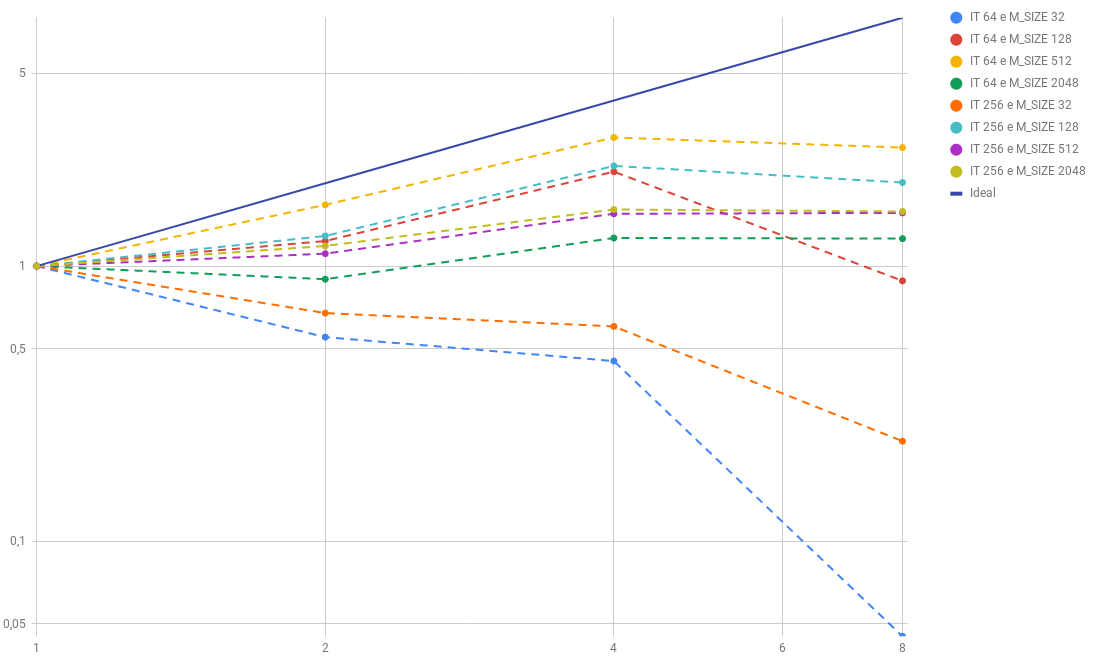
\includegraphics[width=15cm]{Pictures/speedUp.png}
    \label{speedUp}
\end{figure}

Uma constatação imediata mediante observação do gráfico consiste no facto de que, para os casos em que são utilizadas matrizes de pequenas dimensões, o uso de 
\textit{multithreading} não apresenta ganhos apresentando, pelo contrário, uma redução na \textit{performance} obtida. Isto é motivado pelo facto de que a 
criação e sincronização de \textit{threads} anula o ganho obtido com a distribuição de carga pelas mesmas, dado que cada \textit{thread} processa apenas uma fracção
reduzida da matriz.

Por outro lado, denota-se que, para um número de \textit{threads} superior a 4, o ganho obtido diminui, sendo possível verificar uma perda de \textit{performance}
face a versões que recorrem a um número de \textit{threads} menor. Mais uma vez, isto pode ser justificado pelo \textit{overhead} introduzido pela sincronização e 
criação de \textit{threads} bem como pela redução da largura de banda disponível para cada \textit{thread} motivada pela partilha do meio de comunicação.

Por fim, é possível constatar que o número de iterações não influencia o \textit{speed-up} observado afetando apenas o tempo de execução, que é diretamente 
proporcional a este. 

\section{Conclusão} \label{concl}
A presente implementação e análise permite concluir que, o uso de uma API como o OpenMP, torna possível obter ganhos consideráveis em relação à versão sequencial. 

Contudo, isto não dispensa cuidados no que diz respeito ao padrão de acesso à memória que influencia a maneira como a hierarquia de memória é aproveitada, permitindo 
diminuir o número de acessos à memória principal bem como a ocorrência de conflitos na \textit{cache}. Adicionalmente deve ter-se em atenção as otimizações realizadas 
pelo compilador que resultam numa melhoria considerável da \textit{performance} do \textit{kernel}.

Uma observação atenta dos dados permite concluir que a versão paralela, compilada com a \textit{flag} \texttt{-O3} executada em 4 \textit{threads}(uma \textit{thread} por \textit{core}) para \textit{datasets} grandes. Para \textit{datasets} pequenos recomendamos a versão otimizada sequencial apresenta os melhores resultados.

\newpage 

%\onecolumn

\begin{appendices}

\section{Cálculo da Ordem das Matrizes} \label{calOrdem}
\begin{itemize}
    \item Fórmula usada: 
    \begin{equation}
    2\ (matrizes) * ordem\_matriz^{2} = \frac{tamanho\_da\_cache(bytes)}{tamanho\_de\_um\_double(bytes)}
    \end{equation}
    \item \textbf{L1 cache}: 32x32 \newline
        $ 2 * x * x = \frac{32*1024}{8} \Leftrightarrow x \approx 45 $
    \item \textbf{L2 cache}: 128x128 \newline
        $ 2 * x * x = \frac{256*1024}{8} \Leftrightarrow x = 128 $
    \item \textbf{L3 cache}: 512x512 \newline
        $ 2 * x * x = \frac{6144*1024}{8} \Leftrightarrow x \approx 626 $
    \item \textbf{Memória Principal}: 2048x2048 \newline 
        Qualquer matriz de ordem $x$ tal que: \newline $x >= 627 \land 8*x*x*2 <= 8GiB$ \newline (\textbf{i.e.} maior que L3 e que caiba na memória principal) logo: 
        \newline $2*2048*2048*8 = 67108864$ bytes $ \approx 64 MiB$

\end{itemize} 

\section{Baseline vs Optimized} \label{baseVSopt}
\begin{figure}[H]
    \centering
    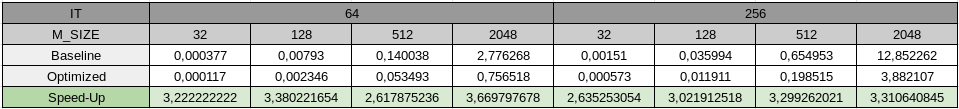
\includegraphics[width=17cm]{Pictures/baseVSopt.png}
\end{figure}

\section{Parallel} \label{parallel}
\begin{figure}[H]
    \centering
    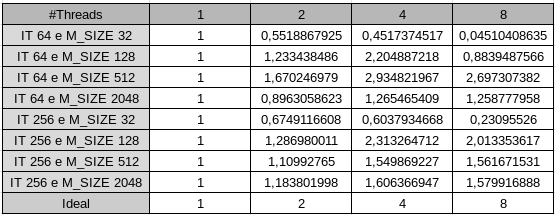
\includegraphics[width=15cm]{Pictures/parallel.png}
\end{figure}

\end{appendices}

\end{document}
